\section{Einrichtung und Entwicklung des ``GReQL Converter''}\label{sec:greql-converter}

Der GReQL Converter stellt eine Webanwendung dar, die es ermöglicht, GReQL-Regeln aus einem UML-Klassendiagramm zu
extrahieren, das mithilfe von PlantText erstellt wurde. Diese extrahierten Regeln dienen anschließend der Bewertung
von UML-Klassendiagrammen auf der JACK-Plattform. Die Realisierung dieser Anwendung erfolgte mit dem Vue.js-Framework
im Frontend und Node.js im Backend, wie in fig-~\ref{fig:infrastructure} veranschaulicht. In diesem Kapitel wird der
Implementierungsprozess der Plattform sowie ihrer verschiedenen Komponenten ausführlich erläutert.

\begin{figure}[h]
    \centering
    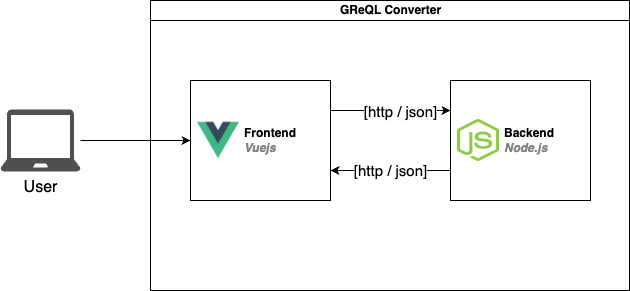
\includegraphics[width=15cm]{images/infrastucture}
    \caption{GReQL-Converter global infrastructure}
    \label{fig:infrastructure}
\end{figure}

\subsection{Einrichtung des PlantUML-Parsers}\label{subsec:einrichtung-des-plantuml-parsers}

Die Entwicklungsphase der Anwendung startete mit der Konfiguration des PlantUML-Parsers. Das ursprüngliche Ziel bestand
darin, eine Anwendung zu entwickeln, die in der Lage ist, PlantText-Code als Eingabe zu akzeptieren und als Ausgabe ein
JSON zu generieren, welches später zur Modellierung von Regelobjekten verwendet werden könnte. Ursprünglich war geplant,
den Parser direkt im Frontend einzusetzen. Es stellte sich jedoch heraus, dass der Parser nur in einer Serverumgebung
effektiv funktioniert. An dieser Stelle gab es zwei Optionen zur Auswahl: die Verwendung eines Tomcat-Servers mit Java
oder eines Node.js-Servers mit JavaScript. Die zweite Option erwies sich als die geeignetere Wahl, da sie es ermöglichte,
dieselbe Programmiersprache für das gesamte Projekt beizubehalten und die Gesamtarchitektur des Systems, einschließlich
seiner zukünftigen Bereitstellung, zu vereinfachen. Node.js eignet sich besonders gut für kleinere Projekte wie dieses.

Im Großen und Ganzen wurde Node.js ausschließlich für die Bereitstellung des Parsers genutzt, was den Backend-Code
erheblich vereinfachte~\ref{lst:bakcend}. Dies ermöglichte einen reibungslosen Übergang zum nächsten Schritt, nämlich
der Erstellung des Grunddesigns der Anwendung.

\subsection{Erstellung des Grunddesigns der Anwendung}\label{subsec:erstellung-des-grunddesigns-der-anwendung}
lorem ipsum.
